
\medskip

 Voici les dimensions de quatre solides: 

\begin{itemize}
\item[$\bullet$] Une pyramide de 6 cm de hauteur dont la base est un rectangle de 6 cm de longueur et de 3 cm de largeur. 

\item[$\bullet$] Un cylindre de 2 cm de rayon et de 3 cm de hauteur. 


\item[$\bullet$] Un cône de 3 cm de rayon et de 3 cm de hauteur. 

\item[$\bullet$] Une boule de 2 cm de rayon. 
\end{itemize}
\parbox{0.55\linewidth}{
\begin{enumerate}
\item

%\begin{enumerate}[a)]
  \begin{enumerate}

\item Représenter approximativement les trois premiers solides comme l'exemple ci-contre : 

\item Placer les dimensions données sur les représentations. 
\end{enumerate}
\item  Classer ces quatre solides dans l'ordre croissant de leur volume. 
\end{enumerate}

}\hfill
 \parbox{0.35\linewidth}{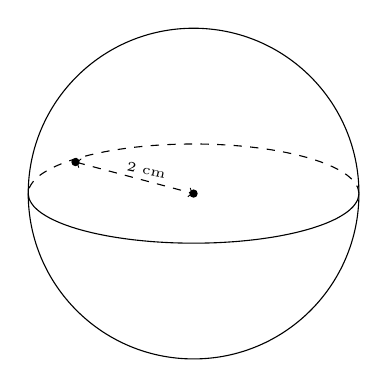
\begin{tikzpicture}[scale=1.5]

  % Paramètres
  \def\rayon{1.4}
  \def\aplati{0.3} % facteur d'écrasement vertical

  % Cercle principal
  \draw (0,0) circle (\rayon);

  % Arc supérieur (ellipse aplatie)
  \draw[dashed, domain=0:180, smooth, variable=\t]
    plot ({\rayon*cos(\t)}, {\rayon*\aplati*sin(\t)});

  % Arc inférieur (ellipse aplatie)
  \draw[domain=180:360, smooth, variable=\t]
    plot ({\rayon*cos(\t)}, {\rayon*\aplati*sin(\t)});

  % Points O et A
  \fill (0,0) circle (1pt) node[below left] {};
  \fill (-1,0.267) circle (1pt) node[above left] {};

  % Ligne AO
  \draw[<->, dashed] (-1,0.267) -- (0,0);

  % Annotation 2 cm, rotation -12°
  \node[rotate=-12] at (-0.4,0.2) {\tiny 2~cm};

\end{tikzpicture}
}


\textit{Quelques formules }: 
$$\dfrac{4}{3}\times \pi\times rayon^3\qquad\hfill\qquad \pi\times rayon^2\times hauteur$$

$$\dfrac{1}{3}\times \pi\times  rayon^2\times hauteur \qquad\hfill\qquad \dfrac{1}{3}\times aire\:de\:la\:base\times hauteur$$




\bigskip

